\chapter{Results}
In order to visually demonstrate the encryption, visualisations of the ciphertext polynomial $c_0$ (refer to \autoref{sec:ckks}) were generated using a CRT decomposition of the RNS representation of $c_0$.
Each pixel corresponds to a coefficient $a \in \Z / q\Z$ scaled down by the modulus $q$ to obtain a brightness value between $0$ and $1$.

\begin{figure}[H]
  \centering
  \pgfplotsset{/pgfplots/group/.cd,vertical sep=1.6cm}
  % This file was created with tikzplotlib v0.10.1.
\begin{tikzpicture}

  \definecolor{darkgray176}{RGB}{176,176,176}
  \definecolor{darkorange25512714}{RGB}{255,127,14}
  \definecolor{lightgray204}{RGB}{204,204,204}
  \definecolor{steelblue31119180}{RGB}{31,119,180}

  \begin{groupplot}[group style={group size=1 by 2}]
    \nextgroupplot[
      height=0.25\linewidth,
      legend cell align={left},
      legend style={
          fill opacity=0.8,
          draw opacity=1,
          text opacity=1,
          at={(0.97,0.03)},
          anchor=south east,
          draw=lightgray204
        },
      tick align=outside,
      tick pos=left,
      width=0.7\linewidth,
      x grid style={darkgray176},
      xlabel={Epochs},
      xmin=0.8, xmax=5.2,
      xtick style={color=black},
      y grid style={darkgray176},
      ylabel={Accuracy},
      ymin=0.902500903606415, ymax=0.985184276103973,
      ytick style={color=black}
    ]
    \addplot [semithick, steelblue31119180]
    table {%
        1 0.90625923871994
        2 0.95637035369873
        3 0.96875923871994
        4 0.976574063301086
        5 0.981425940990448
      };
    \addlegendentry{Training Accuracy}
    \addplot [semithick, darkorange25512714]
    table {%
        1 0.958999991416931
        2 0.967499971389771
        3 0.969833314418793
        4 0.976833343505859
        5 0.97350001335144
      };
    \addlegendentry{Validation Accuracy}

    \nextgroupplot[
      height=0.25\linewidth,
      legend cell align={left},
      legend style={fill opacity=0.8, draw opacity=1, text opacity=1, draw=lightgray204},
      tick align=outside,
      tick pos=left,
      width=0.7\linewidth,
      x grid style={darkgray176},
      xlabel={Epochs},
      xmin=0.8, xmax=5.2,
      xtick style={color=black},
      y grid style={darkgray176},
      ylabel={Loss},
      ymin=0.0464623315259814, ymax=0.342177517153323,
      ytick style={color=black}
    ]
    \addplot [semithick, steelblue31119180]
    table {%
        1 0.328735917806625
        2 0.150406539440155
        3 0.101693823933601
        4 0.0765529051423073
        5 0.0599039308726788
      };
    \addlegendentry{Training Loss}
    \addplot [semithick, darkorange25512714]
    table {%
        1 0.151804178953171
        2 0.107893645763397
        3 0.107302524149418
        4 0.0857750773429871
        5 0.0927918925881386
      };
    \addlegendentry{Validation Loss}
  \end{groupplot}

\end{tikzpicture}

  \caption{Development of the classification accuracy and the mean squared error during training.}
\end{figure}

\begin{figure}[H]
  \centering
  % This file was created with tikzplotlib v0.10.1.
\begin{tikzpicture}[scale=1.2]
  \definecolor{darkgray176}{RGB}{176,176,176}
  \begin{axis}[
      colorbar,
      colorbar style={ylabel={Accuracy}},
      colormap/viridis,
      point meta max=10.1344263202209,
      point meta min=0,
      tick align=outside,
      x grid style={darkgray176},
      xlabel={True Digit},
      xmin=-0.5, xmax=9.5,
      xtick pos=both,
      xtick style={color=black},
      y dir=reverse,
      y grid style={darkgray176},
      ylabel={Classification},
      ymin=-0.5, ymax=9.5,
      ytick pos=left,
      ytick style={color=black}
    ]
    \addplot graphics [includegraphics cmd=\pgfimage,xmin=-0.5, xmax=9.5, ymin=9.5, ymax=-0.5] {../thesis/figures/generated/confusion-matrix-000.png};
    \draw (axis cs:0,0) node[
      scale=0.5,
      text=black,
      rotate=0.0
    ]{963};
    \draw (axis cs:1,0) node[
      scale=0.5,
      text=white,
      rotate=0.0
    ]{0};
    \draw (axis cs:2,0) node[
      scale=0.5,
      text=white,
      rotate=0.0
    ]{2};
    \draw (axis cs:3,0) node[
      scale=0.5,
      text=white,
      rotate=0.0
    ]{2};
    \draw (axis cs:4,0) node[
      scale=0.5,
      text=white,
      rotate=0.0
    ]{0};
    \draw (axis cs:5,0) node[
      scale=0.5,
      text=white,
      rotate=0.0
    ]{1};
    \draw (axis cs:6,0) node[
      scale=0.5,
      text=white,
      rotate=0.0
    ]{8};
    \draw (axis cs:7,0) node[
      scale=0.5,
      text=white,
      rotate=0.0
    ]{3};
    \draw (axis cs:8,0) node[
      scale=0.5,
      text=white,
      rotate=0.0
    ]{1};
    \draw (axis cs:9,0) node[
      scale=0.5,
      text=white,
      rotate=0.0
    ]{0};
    \draw (axis cs:0,1) node[
      scale=0.5,
      text=white,
      rotate=0.0
    ]{0};
    \draw (axis cs:1,1) node[
      scale=0.5,
      text=black,
      rotate=0.0
    ]{1123};
    \draw (axis cs:2,1) node[
      scale=0.5,
      text=white,
      rotate=0.0
    ]{4};
    \draw (axis cs:3,1) node[
      scale=0.5,
      text=white,
      rotate=0.0
    ]{3};
    \draw (axis cs:4,1) node[
      scale=0.5,
      text=white,
      rotate=0.0
    ]{0};
    \draw (axis cs:5,1) node[
      scale=0.5,
      text=white,
      rotate=0.0
    ]{1};
    \draw (axis cs:6,1) node[
      scale=0.5,
      text=white,
      rotate=0.0
    ]{2};
    \draw (axis cs:7,1) node[
      scale=0.5,
      text=white,
      rotate=0.0
    ]{0};
    \draw (axis cs:8,1) node[
      scale=0.5,
      text=white,
      rotate=0.0
    ]{2};
    \draw (axis cs:9,1) node[
      scale=0.5,
      text=white,
      rotate=0.0
    ]{0};
    \draw (axis cs:0,2) node[
      scale=0.5,
      text=white,
      rotate=0.0
    ]{3};
    \draw (axis cs:1,2) node[
      scale=0.5,
      text=white,
      rotate=0.0
    ]{0};
    \draw (axis cs:2,2) node[
      scale=0.5,
      text=black,
      rotate=0.0
    ]{1004};
    \draw (axis cs:3,2) node[
      scale=0.5,
      text=white,
      rotate=0.0
    ]{6};
    \draw (axis cs:4,2) node[
      scale=0.5,
      text=white,
      rotate=0.0
    ]{1};
    \draw (axis cs:5,2) node[
      scale=0.5,
      text=white,
      rotate=0.0
    ]{0};
    \draw (axis cs:6,2) node[
      scale=0.5,
      text=white,
      rotate=0.0
    ]{2};
    \draw (axis cs:7,2) node[
      scale=0.5,
      text=white,
      rotate=0.0
    ]{6};
    \draw (axis cs:8,2) node[
      scale=0.5,
      text=white,
      rotate=0.0
    ]{9};
    \draw (axis cs:9,2) node[
      scale=0.5,
      text=white,
      rotate=0.0
    ]{1};
    \draw (axis cs:0,3) node[
      scale=0.5,
      text=white,
      rotate=0.0
    ]{0};
    \draw (axis cs:1,3) node[
      scale=0.5,
      text=white,
      rotate=0.0
    ]{0};
    \draw (axis cs:2,3) node[
      scale=0.5,
      text=white,
      rotate=0.0
    ]{3};
    \draw (axis cs:3,3) node[
      scale=0.5,
      text=black,
      rotate=0.0
    ]{995};
    \draw (axis cs:4,3) node[
      scale=0.5,
      text=white,
      rotate=0.0
    ]{0};
    \draw (axis cs:5,3) node[
      scale=0.5,
      text=white,
      rotate=0.0
    ]{1};
    \draw (axis cs:6,3) node[
      scale=0.5,
      text=white,
      rotate=0.0
    ]{0};
    \draw (axis cs:7,3) node[
      scale=0.5,
      text=white,
      rotate=0.0
    ]{2};
    \draw (axis cs:8,3) node[
      scale=0.5,
      text=white,
      rotate=0.0
    ]{3};
    \draw (axis cs:9,3) node[
      scale=0.5,
      text=white,
      rotate=0.0
    ]{6};
    \draw (axis cs:0,4) node[
      scale=0.5,
      text=white,
      rotate=0.0
    ]{0};
    \draw (axis cs:1,4) node[
      scale=0.5,
      text=white,
      rotate=0.0
    ]{2};
    \draw (axis cs:2,4) node[
      scale=0.5,
      text=white,
      rotate=0.0
    ]{4};
    \draw (axis cs:3,4) node[
      scale=0.5,
      text=white,
      rotate=0.0
    ]{2};
    \draw (axis cs:4,4) node[
      scale=0.5,
      text=black,
      rotate=0.0
    ]{949};
    \draw (axis cs:5,4) node[
      scale=0.5,
      text=white,
      rotate=0.0
    ]{0};
    \draw (axis cs:6,4) node[
      scale=0.5,
      text=white,
      rotate=0.0
    ]{6};
    \draw (axis cs:7,4) node[
      scale=0.5,
      text=white,
      rotate=0.0
    ]{1};
    \draw (axis cs:8,4) node[
      scale=0.5,
      text=white,
      rotate=0.0
    ]{1};
    \draw (axis cs:9,4) node[
      scale=0.5,
      text=white,
      rotate=0.0
    ]{17};
    \draw (axis cs:0,5) node[
      scale=0.5,
      text=white,
      rotate=0.0
    ]{2};
    \draw (axis cs:1,5) node[
      scale=0.5,
      text=white,
      rotate=0.0
    ]{0};
    \draw (axis cs:2,5) node[
      scale=0.5,
      text=white,
      rotate=0.0
    ]{0};
    \draw (axis cs:3,5) node[
      scale=0.5,
      text=white,
      rotate=0.0
    ]{19};
    \draw (axis cs:4,5) node[
      scale=0.5,
      text=white,
      rotate=0.0
    ]{2};
    \draw (axis cs:5,5) node[
      scale=0.5,
      text=black,
      rotate=0.0
    ]{852};
    \draw (axis cs:6,5) node[
      scale=0.5,
      text=white,
      rotate=0.0
    ]{9};
    \draw (axis cs:7,5) node[
      scale=0.5,
      text=white,
      rotate=0.0
    ]{1};
    \draw (axis cs:8,5) node[
      scale=0.5,
      text=white,
      rotate=0.0
    ]{1};
    \draw (axis cs:9,5) node[
      scale=0.5,
      text=white,
      rotate=0.0
    ]{6};
    \draw (axis cs:0,6) node[
      scale=0.5,
      text=white,
      rotate=0.0
    ]{2};
    \draw (axis cs:1,6) node[
      scale=0.5,
      text=white,
      rotate=0.0
    ]{3};
    \draw (axis cs:2,6) node[
      scale=0.5,
      text=white,
      rotate=0.0
    ]{0};
    \draw (axis cs:3,6) node[
      scale=0.5,
      text=white,
      rotate=0.0
    ]{1};
    \draw (axis cs:4,6) node[
      scale=0.5,
      text=white,
      rotate=0.0
    ]{4};
    \draw (axis cs:5,6) node[
      scale=0.5,
      text=white,
      rotate=0.0
    ]{6};
    \draw (axis cs:6,6) node[
      scale=0.5,
      text=black,
      rotate=0.0
    ]{941};
    \draw (axis cs:7,6) node[
      scale=0.5,
      text=white,
      rotate=0.0
    ]{0};
    \draw (axis cs:8,6) node[
      scale=0.5,
      text=white,
      rotate=0.0
    ]{1};
    \draw (axis cs:9,6) node[
      scale=0.5,
      text=white,
      rotate=0.0
    ]{0};
    \draw (axis cs:0,7) node[
      scale=0.5,
      text=white,
      rotate=0.0
    ]{1};
    \draw (axis cs:1,7) node[
      scale=0.5,
      text=white,
      rotate=0.0
    ]{2};
    \draw (axis cs:2,7) node[
      scale=0.5,
      text=white,
      rotate=0.0
    ]{10};
    \draw (axis cs:3,7) node[
      scale=0.5,
      text=white,
      rotate=0.0
    ]{9};
    \draw (axis cs:4,7) node[
      scale=0.5,
      text=white,
      rotate=0.0
    ]{4};
    \draw (axis cs:5,7) node[
      scale=0.5,
      text=white,
      rotate=0.0
    ]{0};
    \draw (axis cs:6,7) node[
      scale=0.5,
      text=white,
      rotate=0.0
    ]{0};
    \draw (axis cs:7,7) node[
      scale=0.5,
      text=black,
      rotate=0.0
    ]{987};
    \draw (axis cs:8,7) node[
      scale=0.5,
      text=white,
      rotate=0.0
    ]{1};
    \draw (axis cs:9,7) node[
      scale=0.5,
      text=white,
      rotate=0.0
    ]{14};
    \draw (axis cs:0,8) node[
      scale=0.5,
      text=white,
      rotate=0.0
    ]{1};
    \draw (axis cs:1,8) node[
      scale=0.5,
      text=white,
      rotate=0.0
    ]{1};
    \draw (axis cs:2,8) node[
      scale=0.5,
      text=white,
      rotate=0.0
    ]{4};
    \draw (axis cs:3,8) node[
      scale=0.5,
      text=white,
      rotate=0.0
    ]{9};
    \draw (axis cs:4,8) node[
      scale=0.5,
      text=white,
      rotate=0.0
    ]{5};
    \draw (axis cs:5,8) node[
      scale=0.5,
      text=white,
      rotate=0.0
    ]{4};
    \draw (axis cs:6,8) node[
      scale=0.5,
      text=white,
      rotate=0.0
    ]{3};
    \draw (axis cs:7,8) node[
      scale=0.5,
      text=white,
      rotate=0.0
    ]{3};
    \draw (axis cs:8,8) node[
      scale=0.5,
      text=black,
      rotate=0.0
    ]{936};
    \draw (axis cs:9,8) node[
      scale=0.5,
      text=white,
      rotate=0.0
    ]{8};
    \draw (axis cs:0,9) node[
      scale=0.5,
      text=white,
      rotate=0.0
    ]{2};
    \draw (axis cs:1,9) node[
      scale=0.5,
      text=white,
      rotate=0.0
    ]{2};
    \draw (axis cs:2,9) node[
      scale=0.5,
      text=white,
      rotate=0.0
    ]{0};
    \draw (axis cs:3,9) node[
      scale=0.5,
      text=white,
      rotate=0.0
    ]{7};
    \draw (axis cs:4,9) node[
      scale=0.5,
      text=white,
      rotate=0.0
    ]{6};
    \draw (axis cs:5,9) node[
      scale=0.5,
      text=white,
      rotate=0.0
    ]{2};
    \draw (axis cs:6,9) node[
      scale=0.5,
      text=white,
      rotate=0.0
    ]{0};
    \draw (axis cs:7,9) node[
      scale=0.5,
      text=white,
      rotate=0.0
    ]{3};
    \draw (axis cs:8,9) node[
      scale=0.5,
      text=white,
      rotate=0.0
    ]{1};
    \draw (axis cs:9,9) node[
      scale=0.5,
      text=black,
      rotate=0.0
    ]{986};
  \end{axis}

\end{tikzpicture}

  \caption{Confusion Matrix of the trained network.}
\end{figure}

\begin{figure}[H]
  \centering
  % 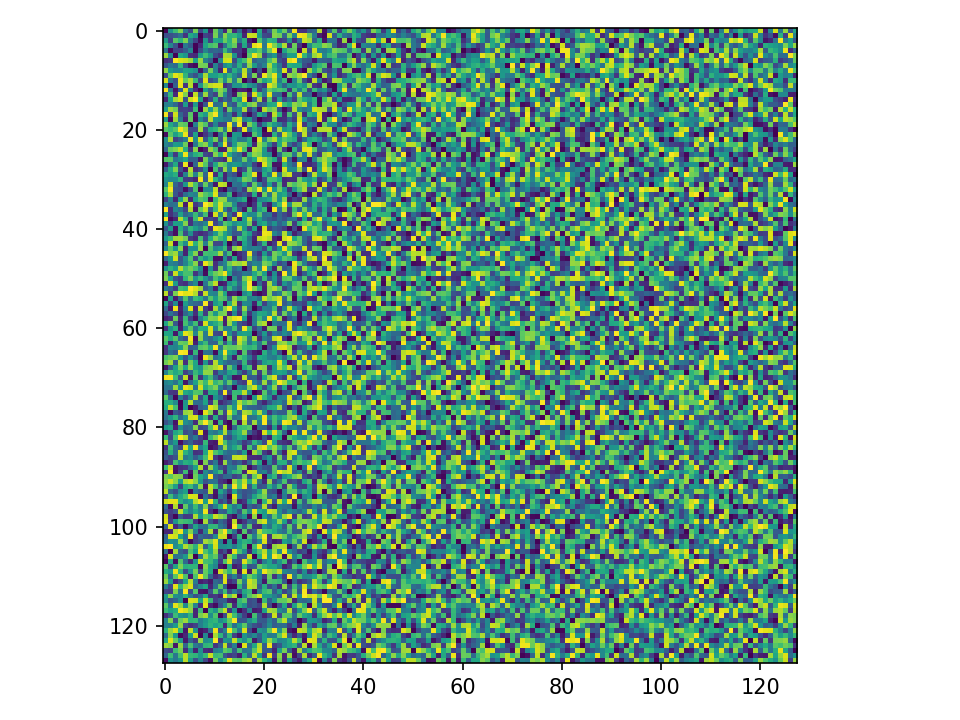
\includegraphics[width=\linewidth]{figures/ciphertext-visualisation.png}
  \pgfplotsset{/pgfplots/group/.cd,vertical sep=0.3cm,horizontal sep=0.3cm}
  % This file was created with tikzplotlib v0.10.1.
\def\ciphertextimagesize{0.25\linewidth}
\begin{tikzpicture}
  \definecolor{darkgray176}{RGB}{176,176,176}
  \begin{groupplot}[group style={group size=5 by 2}]
    \nextgroupplot[
      height=\ciphertextimagesize,
      hide x axis,
      hide y axis,
      tick align=outside,
      tick pos=left,
      width=\ciphertextimagesize,
      x grid style={darkgray176},
      xmin=-0.5, xmax=27.5,
      xtick style={color=black},
      y dir=reverse,
      y grid style={darkgray176},
      ymin=-0.5, ymax=27.5,
      ytick style={color=black}
    ]
    \addplot graphics [includegraphics cmd=\pgfimage,xmin=-0.5, xmax=27.5, ymin=27.5, ymax=-0.5] {figures/generated/ciphertext-visualisation-000.png};

    \nextgroupplot[
      height=\ciphertextimagesize,
      hide x axis,
      hide y axis,
      tick align=outside,
      tick pos=left,
      width=\ciphertextimagesize,
      x grid style={darkgray176},
      xmin=-0.5, xmax=127.5,
      xtick style={color=black},
      y dir=reverse,
      y grid style={darkgray176},
      ymin=-0.5, ymax=127.5,
      ytick style={color=black}
    ]
    \addplot graphics [includegraphics cmd=\pgfimage,xmin=-0.5, xmax=127.5, ymin=127.5, ymax=-0.5] {figures/generated/ciphertext-visualisation-001.png};

    \nextgroupplot[
      height=\ciphertextimagesize,
      hide x axis,
      hide y axis,
      tick align=outside,
      tick pos=left,
      width=\ciphertextimagesize,
      x grid style={darkgray176},
      xmin=-0.5, xmax=27.5,
      xtick style={color=black},
      y dir=reverse,
      y grid style={darkgray176},
      ymin=-0.5, ymax=27.5,
      ytick style={color=black}
    ]
    \addplot graphics [includegraphics cmd=\pgfimage,xmin=-0.5, xmax=27.5, ymin=27.5, ymax=-0.5] {figures/generated/ciphertext-visualisation-002.png};

    \nextgroupplot[
      height=\ciphertextimagesize,
      hide x axis,
      hide y axis,
      tick align=outside,
      tick pos=left,
      width=\ciphertextimagesize,
      x grid style={darkgray176},
      xmin=-0.5, xmax=127.5,
      xtick style={color=black},
      y dir=reverse,
      y grid style={darkgray176},
      ymin=-0.5, ymax=127.5,
      ytick style={color=black}
    ]
    \addplot graphics [includegraphics cmd=\pgfimage,xmin=-0.5, xmax=127.5, ymin=127.5, ymax=-0.5] {figures/generated/ciphertext-visualisation-003.png};

    \nextgroupplot[
      height=\ciphertextimagesize,
      hide x axis,
      hide y axis,
      tick align=outside,
      tick pos=left,
      width=\ciphertextimagesize,
      x grid style={darkgray176},
      xmin=-0.5, xmax=27.5,
      xtick style={color=black},
      y dir=reverse,
      y grid style={darkgray176},
      ymin=-0.5, ymax=27.5,
      ytick style={color=black}
    ]
    \addplot graphics [includegraphics cmd=\pgfimage,xmin=-0.5, xmax=27.5, ymin=27.5, ymax=-0.5] {figures/generated/ciphertext-visualisation-004.png};

    \nextgroupplot[
      height=\ciphertextimagesize,
      hide x axis,
      hide y axis,
      tick align=outside,
      tick pos=left,
      width=\ciphertextimagesize,
      x grid style={darkgray176},
      xmin=-0.5, xmax=127.5,
      xtick style={color=black},
      y dir=reverse,
      y grid style={darkgray176},
      ymin=-0.5, ymax=127.5,
      ytick style={color=black}
    ]
    \addplot graphics [includegraphics cmd=\pgfimage,xmin=-0.5, xmax=127.5, ymin=127.5, ymax=-0.5] {figures/generated/ciphertext-visualisation-005.png};

    \nextgroupplot[
      height=\ciphertextimagesize,
      hide x axis,
      hide y axis,
      tick align=outside,
      tick pos=left,
      width=\ciphertextimagesize,
      x grid style={darkgray176},
      xmin=-0.5, xmax=27.5,
      xtick style={color=black},
      y dir=reverse,
      y grid style={darkgray176},
      ymin=-0.5, ymax=27.5,
      ytick style={color=black}
    ]
    \addplot graphics [includegraphics cmd=\pgfimage,xmin=-0.5, xmax=27.5, ymin=27.5, ymax=-0.5] {figures/generated/ciphertext-visualisation-006.png};

    \nextgroupplot[
      height=\ciphertextimagesize,
      hide x axis,
      hide y axis,
      tick align=outside,
      tick pos=left,
      width=\ciphertextimagesize,
      x grid style={darkgray176},
      xmin=-0.5, xmax=127.5,
      xtick style={color=black},
      y dir=reverse,
      y grid style={darkgray176},
      ymin=-0.5, ymax=127.5,
      ytick style={color=black}
    ]
    \addplot graphics [includegraphics cmd=\pgfimage,xmin=-0.5, xmax=127.5, ymin=127.5, ymax=-0.5] {figures/generated/ciphertext-visualisation-007.png};

    \nextgroupplot[
      height=\ciphertextimagesize,
      hide x axis,
      hide y axis,
      tick align=outside,
      tick pos=left,
      width=\ciphertextimagesize,
      x grid style={darkgray176},
      xmin=-0.5, xmax=27.5,
      xtick style={color=black},
      y dir=reverse,
      y grid style={darkgray176},
      ymin=-0.5, ymax=27.5,
      ytick style={color=black}
    ]
    \addplot graphics [includegraphics cmd=\pgfimage,xmin=-0.5, xmax=27.5, ymin=27.5, ymax=-0.5] {figures/generated/ciphertext-visualisation-008.png};

    \nextgroupplot[
      height=\ciphertextimagesize,
      hide x axis,
      hide y axis,
      tick align=outside,
      tick pos=left,
      width=\ciphertextimagesize,
      x grid style={darkgray176},
      xmin=-0.5, xmax=127.5,
      xtick style={color=black},
      y dir=reverse,
      y grid style={darkgray176},
      ymin=-0.5, ymax=127.5,
      ytick style={color=black}
    ]
    \addplot graphics [includegraphics cmd=\pgfimage,xmin=-0.5, xmax=127.5, ymin=127.5, ymax=-0.5] {figures/generated/ciphertext-visualisation-009.png};
  \end{groupplot}
\end{tikzpicture}

  \caption{Ciphertext Visualisation}
\end{figure}

\section{Methodology}

\section{Accuracy, Precision, Recall}
% Detailliertere Analyse
% https://medium.com/analytics-vidhya/accuracy-precision-and-recall-in-machine-learning-classification-ae84004e86a1
% https://en.wikipedia.org/wiki/Precision_and_recall

\section{Performance Benchmarks}
This chapter includes runtime and communication overhead analysis.

Plain runtime: xxx

\begin{table}[H]
  \centering
  \caption{Performance Benchmarks / Communication Overhead}
  \begin{tabular}{lllll}
    \textbf{Scenario} & \textbf{Parameters} & \textbf{Runtime} / \si{\second} & \textbf{Message Size} / \si{\mega\byte} & \textbf{MRE} \\
    BSGS Matmul       & 60,40,...,40,60     &                                 &                                         &              \\
    BSGS Matmul       & 34,25,...,25,34     &                                 &                                         &              \\
    Hybrid Matmul     &                     &                                 &                                         &              \\
    Encrypt           &                     &                                 &                                         &              \\
    Encrypt Symmetric &                     &                                 &                                         &              \\
  \end{tabular}
\end{table}
